% ==================== 2.4.2 三重旋转轴 ====================
\subsubsection{三重旋转轴（\texorpdfstring{$P\,3$}{P3}）}

旋转轴 $n$ 是一条几何直线：晶体绕它每转 $2\pi/n$ 就复原，转满 $n$ 次后原子回到原处。
要观察 3 次轴，可选用 $c$ 轴为 3 次轴的空间群 $P\,3$（No.~143，三方晶系）；晶胞参数
与原子坐标见表~\ref{tab:sym-rot3}。

\begin{table}[H]
  \centering
  \caption{三重旋转轴演示的建模参数}
  \label{tab:sym-rot3}
  \begin{tabular}{ll}
    \toprule
    项目 & 参数 \\
    \midrule
    空间群 & $P\,3$（No.~143，三方晶系） \\
    晶格常数 & $a=b=c=2.0$\,\AA，$\alpha=\beta=90^\circ$，$\gamma=120^\circ$ \\
    原子坐标 & Si：$(0.2,\,0.3,\,0.4)$（一般位置） \\
    等效位置数 & 3（单胞内 3 个原子） \\
    \bottomrule
  \end{tabular}
\end{table}

\begin{figure}[H]
  \centering
  \subcaptionbox{空间群与晶胞参数设置}{%
    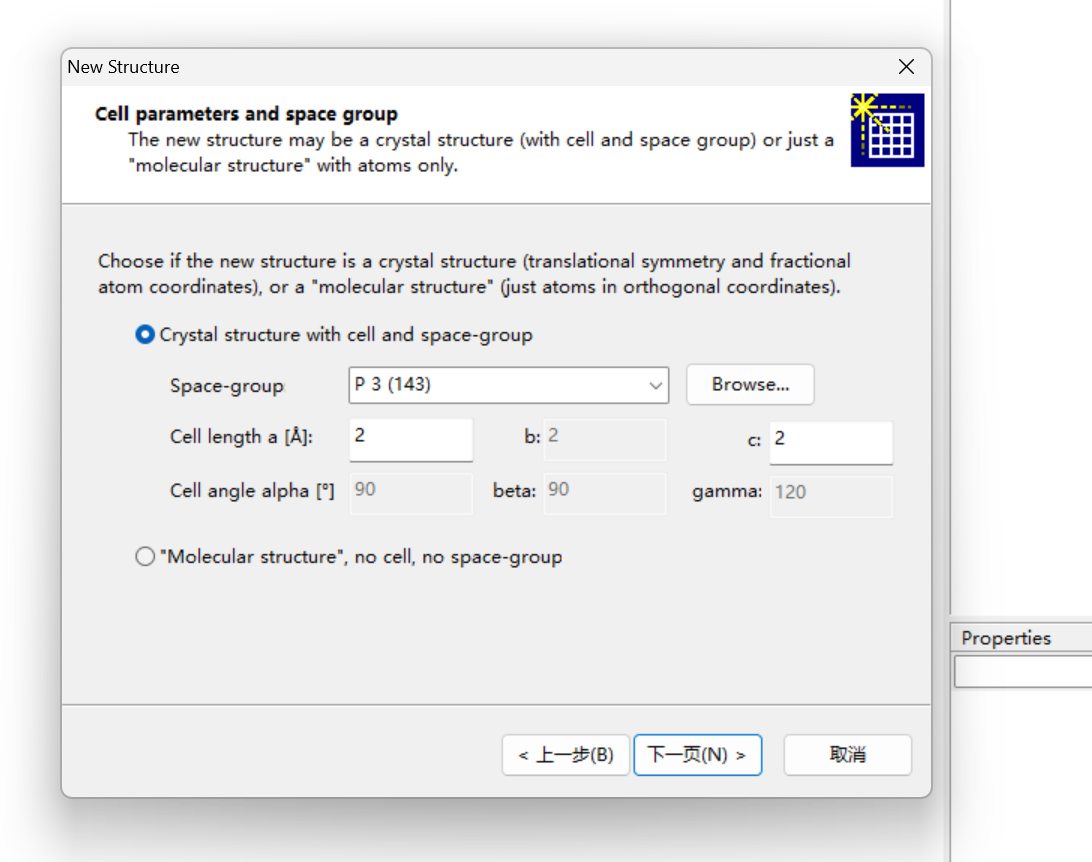
\includegraphics[width=0.44\textwidth]{assets/symmetry/rotation3/a.png}}
  \hfill
  \subcaptionbox{非对称单元原子（Si）添加}{%
    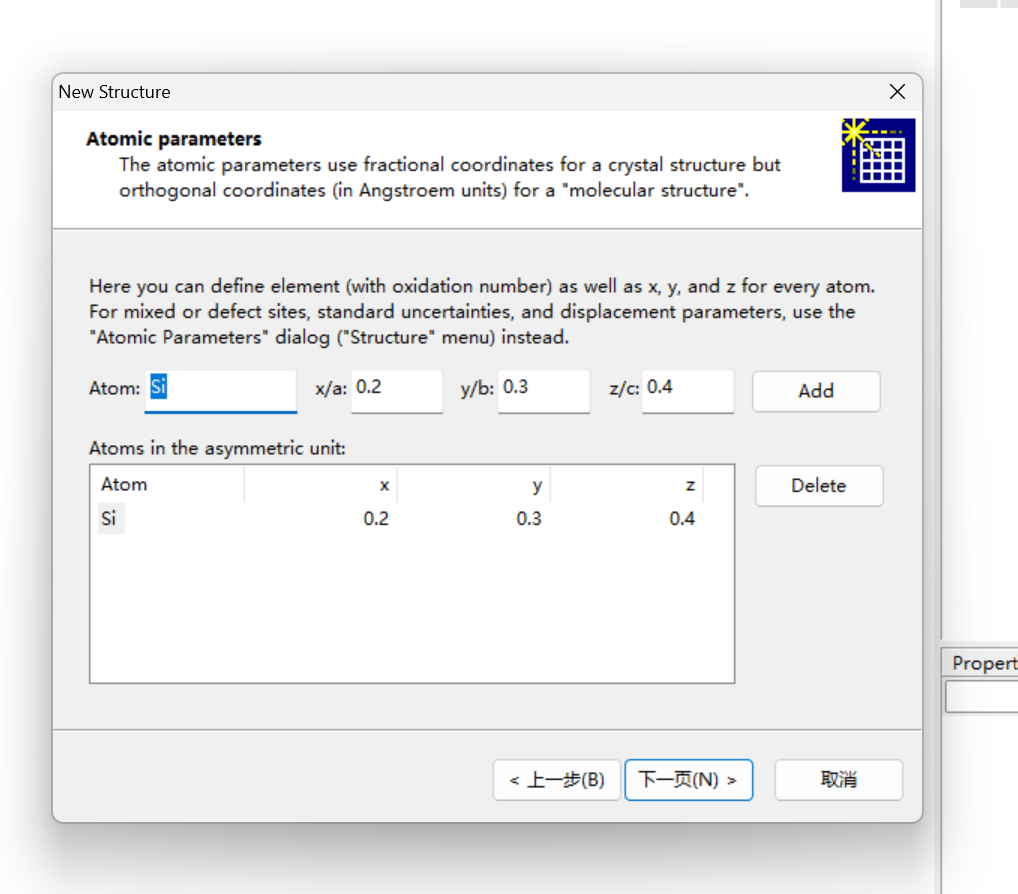
\includegraphics[width=0.44\textwidth]{assets/symmetry/rotation3/b.png}}
  \caption{三重旋转轴（$P\,3$）演示的参数设置}
  \label{fig:sym-rot3-param}
\end{figure}

\begin{figure}[H]
  \centering
  \subcaptionbox{单胞图：3 个原子绕 $c$ 轴呈 $120^\circ$ 分布、位于同一平面}{%
    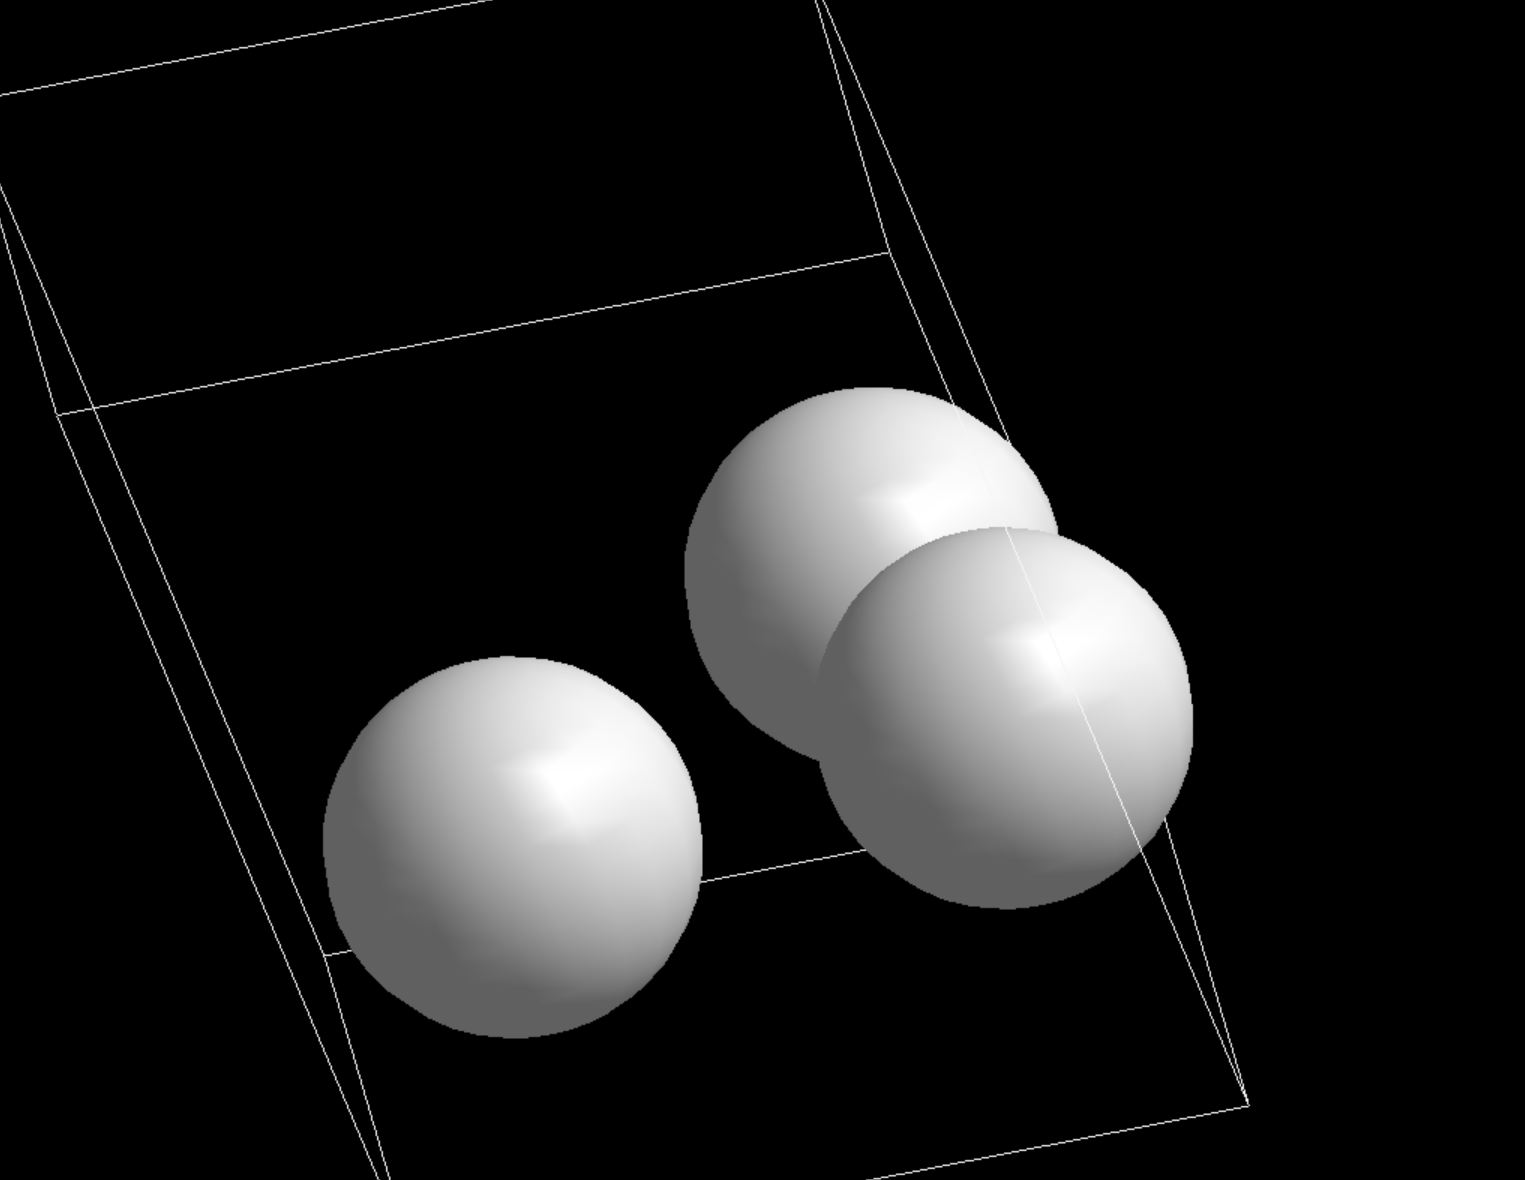
\includegraphics[width=0.44\textwidth]{assets/symmetry/rotation3/c.png}}
  \hfill
  \subcaptionbox{超晶胞图：三重对称花样的周期复现}{%
    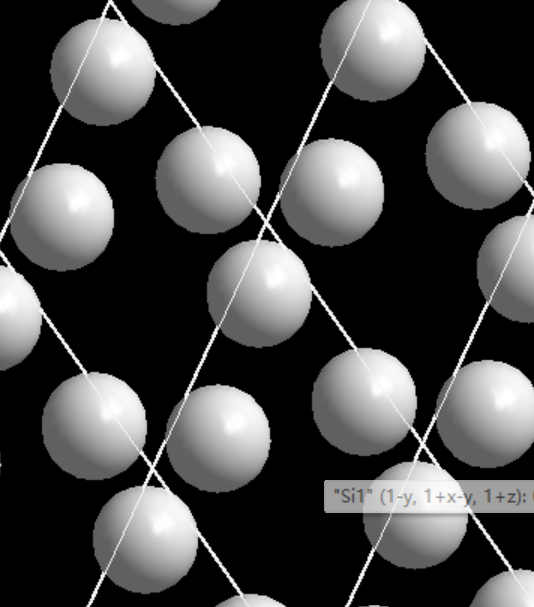
\includegraphics[width=0.44\textwidth]{assets/symmetry/rotation3/d.png}}
  \caption{三重旋转轴（$P\,3$）的单胞与超晶胞模型}
  \label{fig:sym-rot3-model}
\end{figure}

$P\,3$ 的一般位置等效位置为 $(x,y,z)$、$(\bar y,\,x-y,\,z)$ 与 $(-x+y,\,\bar x,\,z)$，
即每次绕 $c$ 轴旋转 $120^\circ$ 得到下一个原子，旋转三次后回到初始位置。将 Si 的
坐标 $(0.2,0.3,0.4)$ 代入，三个原子的分数坐标为 $(0.2,0.3,0.4)$、$(0.7,0.9,0.4)$ 与
$(0.1,0.8,0.4)$：三者 $z$ 坐标相同，位于垂直于 $c$ 轴的同一平面内，且绕 $c$ 轴依次
相距 $120^\circ$（图~\ref{fig:sym-rot3-model}(a)）；在超晶胞中，三重对称花样
沿各方向周期复现（图~\ref{fig:sym-rot3-model}(b)）。

\textbf{一个容易混淆的对照。}$n$ 重旋转轴给出 $n$ 个等效原子，且全部落在垂直于轴的
同一平面内。受晶格周期性限制，晶体中只可能存在 1、2、3、4、6 次旋转轴（见
2.2.2 节），3 次轴是三方晶系的特征对称元素。要注意的是，由旋转轴联系起来的原子只有
``绕轴旋转''的关系，不涉及沿轴方向的平移；把这层关系再加上一个平移分量，得到的就是
2.4.5 节要演示的螺旋轴。
